
\chapter{Chapter 2. Background and Related Work}

This chapter covers the technical background for this thesis. Section~\ref{sec:biencoder} describes the bi-encoder architecture for dense retrieval and the three models we used. Section~\ref{sec:contrastive} introduces the contrastive learning objective for training the embedding model. Section~\ref{sec:compression_bg} covers the embedding compression techniques. In Section~\ref{sec:ir_eval}, we define the evaluation metrics and the significance test. And finally, Section~\ref{sec:related} looks at the related work and positions this thesis relative to previous contributions.

\section{Dense Retrieval with Bi-Encoders}
\label{sec:biencoder}

\subsection{Transformer Encoders}

Modern dense retrieval systems are built on top of transformer-based language models~\cite{devlin2019bert}. A transformer encoder maps a token sequence of length $L$ to a sequence of contextualized hidden states $\mathbf{H} \in \mathbb{R}^{L \times d_h}$, where $d_h$ is the hidden dimension, through a stack of self-attention and feed-forward layers. Each self-attention layer allows every token to attend to every other token in the sequence, producing representations that capture long-range syntactic and semantic dependencies. Bidirectional encoders such as BERT (Bidirectional Encoder Representations from Transformers)~\cite{devlin2019bert} are pre-trained on large text corpora via masked language modeling (MLM), yielding general-purpose representations that transfer well to downstream tasks with minimal task-specific fine-tuning.

\subsection{Bi-Encoder Architecture}

\begin{figure}[!h]
  \centering
  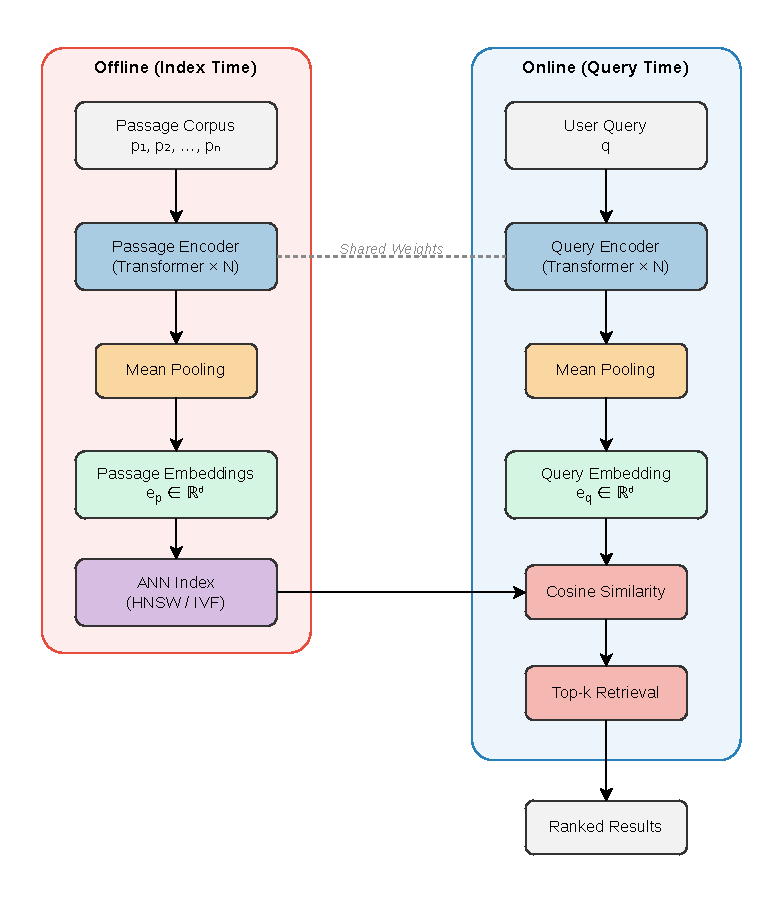
\includegraphics[width=0.85\textwidth]{Figures/biencoder_arch.pdf}
  \caption[Bi-encoder retrieval architecture.]{Bi-encoder retrieval architecture. Everything in the corpus is encoded and saved in an ANN index at index time (left). At query time (on the right), the query is encoded and compared to the index using cosine similarity to find the $k$ most relevant passages. Weights are shared by both encoders.}
  \label{fig:biencoder}
\end{figure}

A bi-encoder, sometimes called a dual encoder, is made up of two transformer encoders: one for passages and one for queries. The outputs of these two encoders are compressed into dense vectors of fixed size~\cite{reimers2019sbert, karpukhin2020dense}. The full bi-encoder retrieval process is shown in Figure~\ref{fig:biencoder}. Most of the time, the two towers share weights. There is a separate encoder for each question ($q$) and passage ($p$). Each query $q$ and passage $p$ are encoded independently:
%
\begin{equation}
  \mathbf{e}_q = \text{pool}(\text{Enc}(q)), \qquad \mathbf{e}_p = \text{pool}(\text{Enc}(p)),
\end{equation}
%
where $\text{pool}(\cdot)$ is a pooling operation applied to the set of hidden states.
Sentence-BERT (SBERT)~\cite{reimers2019sbert} established mean pooling as a standard for retrieval models. Relevance is computed using cosine similarity between the query and passage embeddings:
%
\begin{equation}
  \text{sim}(\mathbf{e}_q, \mathbf{e}_p) = \frac{\mathbf{e}_q \cdot \mathbf{e}_p}{\|\mathbf{e}_q\| \|\mathbf{e}_p\|}.
\end{equation}
%
Separating the query and passage encoding is a key feature of bi-encoders for large-scale retrieval. Passage embeddings can be calculated offline and stored in an approximate nearest-neighbor (ANN) index. This way, only the query encoder runs at query time, and retrieval is reduced to a single nearest-neighbor lookup~\cite{karpukhin2020dense}. Cross-encoders, on the other hand, jointly encode both the query and passage and hence cannot precompute a representation.

For an exact exhaustive search, each query is compared against all passage vectors. This takes $\mathcal{O}(N \cdot d)$ time. Here, $N$ is the number of passages and $d$ is the embedding dimension.

Take, for example, 10 million passages each with 768-dimensional embeddings. Computing relevant passages for a query takes about 15 billion floating-point operations. This makes a latency of less than 1 millisecond unachievable. Hierarchical Navigable Small World (HNSW)~\cite{malkov2018efficient} and Inverted File Index (IVF)~\cite{johnson2021billion} are two ANN indices that address this problem. They do this by organizing vectors so that only a small part of the corpus needs visiting. This gets the speed back with a small loss in recall. Specialized disk-resident indices like DiskANN~\cite{subramanya2019diskann} lower this memory need even more by using SSDs to improve graph traversal. But their latency is roughly three orders of magnitude slower than that of DRAM. Hence, in-memory indexing is preferred for interactive workloads. Even with ANN indexing, most applications need the full set of passage embeddings in memory. This thesis gets around the memory problem by compressing the embeddings.

\subsection{Backbone Models}

This thesis evaluates compression methods across three backbone encoders to test whether the compression technique is effective and if it generalizes for different backbones or not.

\textbf{BGE-base-en-v1.5}~\cite{xiao2023c} is the primary backbone for this thesis. BGE (BAAI General Embedding) is a family of English bi-encoders from the Beijing Academy of Artificial Intelligence (BAAI). The base variant was chosen because it had strong performance on the Massive Text Embedding Benchmark (MTEB)~\cite{muennighoff2022mteb} at moderate parameter count.

\begin{table}[H]
  \centering
  \caption[Backbone encoder models used in this thesis]{Backbone encoder models. All three of them use a 12-layer transformer block and produce 768-dimensional float32 embeddings by mean pooling.}
  \label{tab:backbones}
  \begin{tabular}{| l | c | l |}
    \hline
    \textbf{Model} & \textbf{Parameters} & \textbf{Pre-training Strategy} \\ [0.5ex] \hline
    BGE-base-en-v1.5~\cite{xiao2023c}    & 109M & MLM + retrieval fine-tuning \\ \hline
    RoBERTa-base~\cite{liu2019roberta}   & 125M & Optimized MLM \\ \hline
    MPNet-base~\cite{song2020mpnet}      & 110M & Masked + permuted LM \\ \hline
  \end{tabular}
\end{table}

\textbf{RoBERTa-base} (Robustly Optimized BERT Pretraining Approach)~\cite{liu2019roberta} is a replication study of BERT that corrects many under-training choices. It gets rid of the Next Sentence Prediction (NSP) objective, uses dynamic masks, bigger batch sizes, and 10 times more training data. Even though the architecture stays the same, these changes make the representations better on standard NLU benchmarks~\cite{wang2018glue, rajpurkar2016squad}.

\textbf{MPNet-base} (Masked and Permuted Pre-training)~\cite{song2020mpnet} combines masked language modeling with permuted language modeling. When BERT predicts a masked token, it ignores other masked places. MPNet, on the other hand, predicts tokens autoregressively in a random permutation order while paying attention to the whole sequence. This way, it finds dependencies between masked tokens that MLM-only models miss. The MPNet pre-training objective is different from both BERT and BGE. This helps test the generalizability of the compression results even more.

The three backbones have different starting retrieval quality. BGE is the best place to start because it comes already fine-tuned for retrieval. MPNet has an intermediate starting point because of its masked and permuted goal. RoBERTa has the weakest initial retrieval representations because it was only taught on the MLM task. This order (BGE $>$ MPNet $>$ RoBERTa) is also confirmed by the zero-shot NanoBEIR baselines reported in Chapter~4. With these different qualities of backbones, we are trying to answer whether the property of compression trade-offs stays the same or not.

\section{Contrastive Learning for Dense Retrieval}
\label{sec:contrastive}

Contrastive learning teaches a model to put things that are semantically related close to each other, and things that are not, far apart~\cite{oord2018representation}. In the Information Noise-Contrastive Estimation (InfoNCE) loss, this is turned into an $N$-way classification task: the model has to give the positive pair the highest similarity score among the $N{-}1$ negatives.

Multiple Negatives Ranking Loss (MNRL) is the in-batch implementation of InfoNCE used by the sentence-transformers system~\cite{reimers2019sbert}. It is used in this thesis. The negatives are obtained for free from other examples within the batch. For a batch of $N$ positive query-passage pairs $\{(q_i, p_i^+)\}_{i=1}^{N}$, the positive passage of other pairs acts as a negative for query $q_i$ (Figure~\ref{fig:mnrl}).

\begin{figure}[!h]
  \centering
  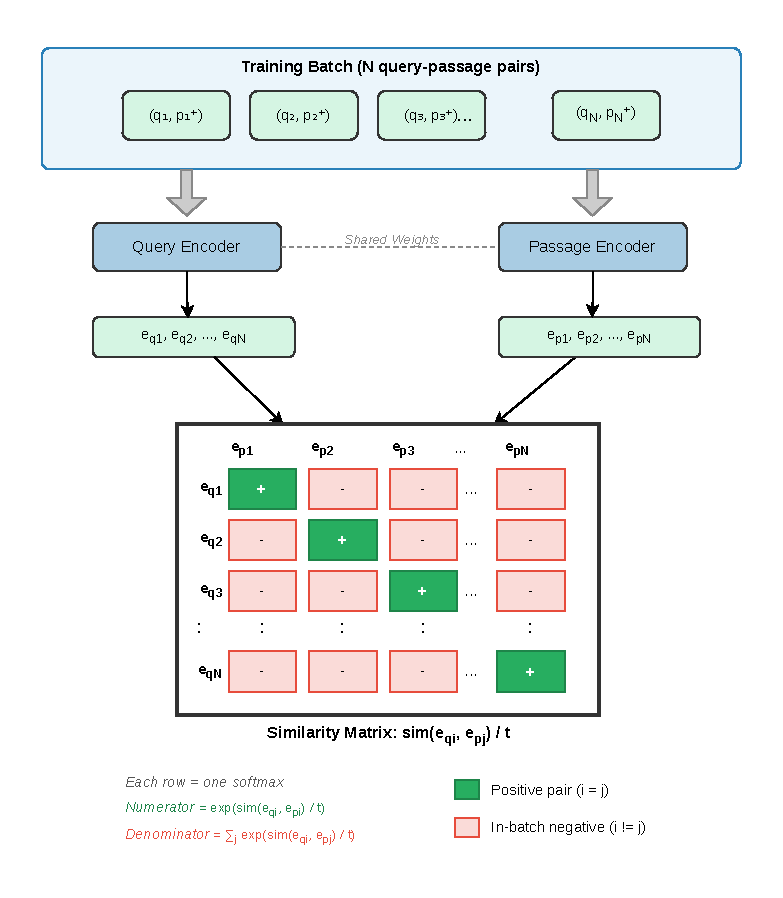
\includegraphics[width=0.85\textwidth]{Figures/mnrl_loss.pdf}
  \caption[Multiple Negatives Ranking Loss (MNRL).]{Multiple Negatives Ranking Loss. A training batch of $N$ pairs is encoded by the shared weights. The $N \times N$ similarity matrix scores every query against every passage in the batch. The loss is made up of positive pairs on the diagonal (green), in the numerator. The denominator is made up of each full row, which makes each row an $N$-way softmax classification.}
  \label{fig:mnrl}
\end{figure}

The loss for the full batch is:
%
\begin{equation}
  \mathcal{L}_{\text{MNRL}} = -\frac{1}{N} \sum_{i=1}^{N} \log \frac{\exp\!\left(\text{sim}(\mathbf{e}_{q_i}, \mathbf{e}_{p_i^+}) / \tau\right)}{\sum_{j=1}^{N} \exp\!\left(\text{sim}(\mathbf{e}_{q_i}, \mathbf{e}_{p_j^+}) / \tau\right)},
  \label{eq:mnrl}
\end{equation}
%
where $\tau > 0$ is a temperature hyperparameter that controls how peaked the softmax distribution is. In-batch negatives are effective because large batch sizes expose each query to many diverse negatives simultaneously. Also, batch mates are often related by topic to the query, providing challenging but informative negatives without any explicit negative mining~\cite{karpukhin2020dense}.

\section{Embedding Compression Methods}
\label{sec:compression_bg}

This thesis organizes embedding compression methods along two orthogonal axes. The first axis is when compression is applied. Post-hoc compression methods are applied to the embeddings generated by the models that weren't modified. But training-time methods incorporate compression awareness into the model's fine-tuning objective. The second axis is how the memory requirement is reduced. We can reduce precision of embeddings by decreasing the number of bits per dimension, we can truncate embedding dimensions, or we can learn a hash that fits a codebook mapping embeddings to discrete codes. Table~\ref{tab:compression-taxonomy} presents the methods studied in this thesis along these two axes.

\begin{table}[H]
  \centering
  \caption[Organization of embedding compression methods studied in this thesis]{Organization of embedding compression methods based on when and how compression is applied. Abbreviations: INT8 = 8-bit integer quantization; PQ = Product Quantization; BAT = Binarization-Aware Training (STE and Annealed Tanh are two training variants); STE = Straight-Through Estimator; MRL = Matryoshka Representation Learning.}
  \label{tab:compression-taxonomy}
  \begin{tabular}{| l | c | c | c |}
    \hline
                            & \textbf{Precision Reduction} & \textbf{Dim.\ Reduction} & \textbf{Learning to Hash} \\ [0.5ex] \hline
    \textbf{Post-hoc}       & INT8, Binary, TurboQuant     & ---                      & PQ                        \\ \hline
    \textbf{Training-time}  & BAT (STE / Annealed Tanh)    & MRL                      & ---                       \\ \hline
  \end{tabular}
\end{table}

The classification in Table~\ref{tab:compression-taxonomy} reflects when training is modified, not when the compressed representation is produced. At retrieval time, all of the methods do something: truncation, sign-thresholding, or scalar quantization. For post-hoc methods, this retrieval time operation is the entire compression step, applied to a model that was not trained for it. For training-time methods, the same kind of operation is still required at retrieval (taking the sign of a BAT embedding, truncating an MRL embedding to its first $m$ dimensions). But they are effective because training was modified to make that operation lossy in a controlled way rather than destructive.

The following subsections describe each method, grouped by when compression is applied.

\subsection{Post-hoc Methods}

\subsubsection{Scalar Quantization}

\begin{figure}[!h]
  \centering
  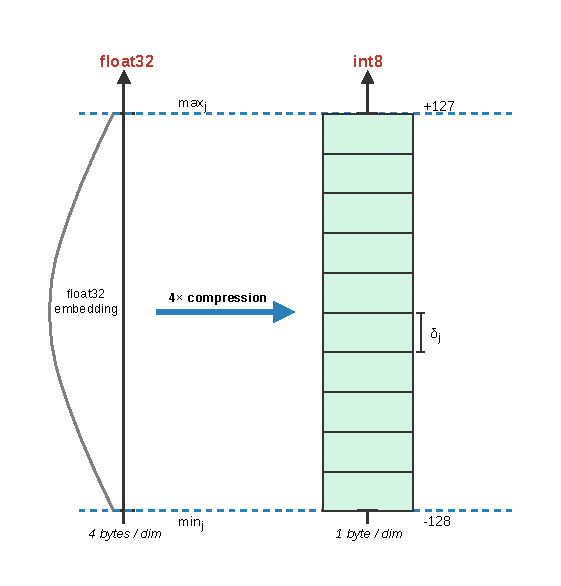
\includegraphics[width=0.75\textwidth]{Figures/scalar_quant.pdf}
  \caption[Scalar quantization of a single embedding dimension.]{Scalar quantization of a single embedding dimension. The float32 value $x$ (left) is mapped to a signed 8-bit integer $x_q \in [-128, 127]$ (right) using 256 uniform quantization levels of width $\delta_j$, and per-dimension calibration range $[\min_j, \max_j]$.}
  \label{fig:scalar_quant}
\end{figure}

As shown in Figure~\ref{fig:scalar_quant}, scalar quantization maps each float32 value to a lower-precision number. To find the lower and upper limits $[\min_j, \max_j]$ for INT8 quantization, we need a calibration subset. Here, $j$ is the index for the embedding dimension.
Embedding value $x$ at index $j$ is then quantized as:
%
\begin{equation}
  x_q = \left\lfloor \frac{x - \min_j}{\delta_j} \right\rceil - 128,
  \qquad \delta_j = \frac{\max_j - \min_j}{255},
  \label{eq:int8}
\end{equation}
%
where $\lfloor \cdot \rceil$ denotes rounding to the nearest integer, and the $-128$ shift turns the unsigned range $[0, 255]$ into the signed 8-bit range $[-128, 127]$.
It cuts storage from 4 bytes per dimension to 1 byte per dimension ($4\times$ compression) by using all 256 levels across the recorded range of each dimension~\cite{douze2024faiss}.

\subsubsection{Binary Quantization}

\begin{figure}[!h]
  \centering
  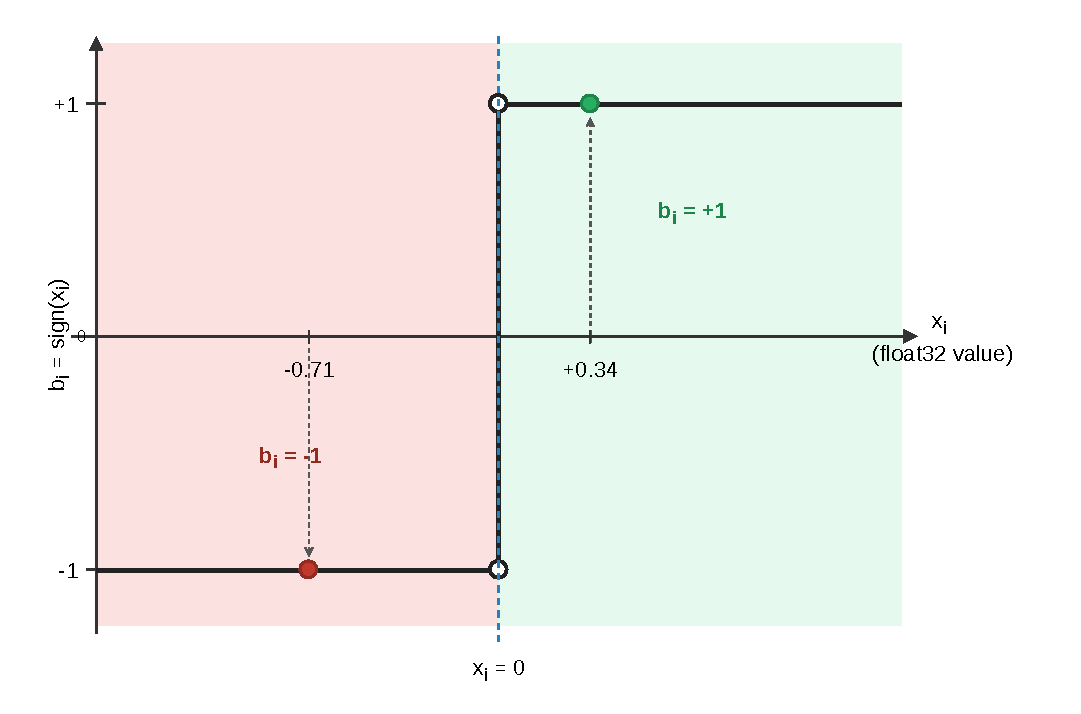
\includegraphics[width=0.75\textwidth]{Figures/step_function.pdf}
  \caption[Binary quantization via the sign function.]{Binary quantization maps each float32 embedding dimension $x_i$ to a binary value $b_i \in \{-1, +1\}$ with the sign function. All positive values map to $+1$ (green region) and all negative values map to $-1$ (red region).}
  \label{fig:binary_quant}
\end{figure}

By using the sign function, binary quantization changes each float32 value to a single bit, as shown in Figure~\ref{fig:binary_quant}:
%
\begin{equation}
  b_i = \text{sign}(x_i) \in \{-1, +1\},
\end{equation}
%
where $x_i$ is the $i$-th dimension of the float32 embedding and $b_i$ is the corresponding bit. This gives a $32\times$ compression over float32. The Hamming distance is used to find the similarity between a binary query vector $\mathbf{b}_q$ and a passage vector $\mathbf{b}_p$.
In modern hardware, the Hamming distance can be reduced to bitwise XOR followed by popcount, which can be much faster than cosine similarity computation~\cite{gan2023binary}.

\subsubsection{Product Quantization}

\begin{figure}[!h]
  \centering
  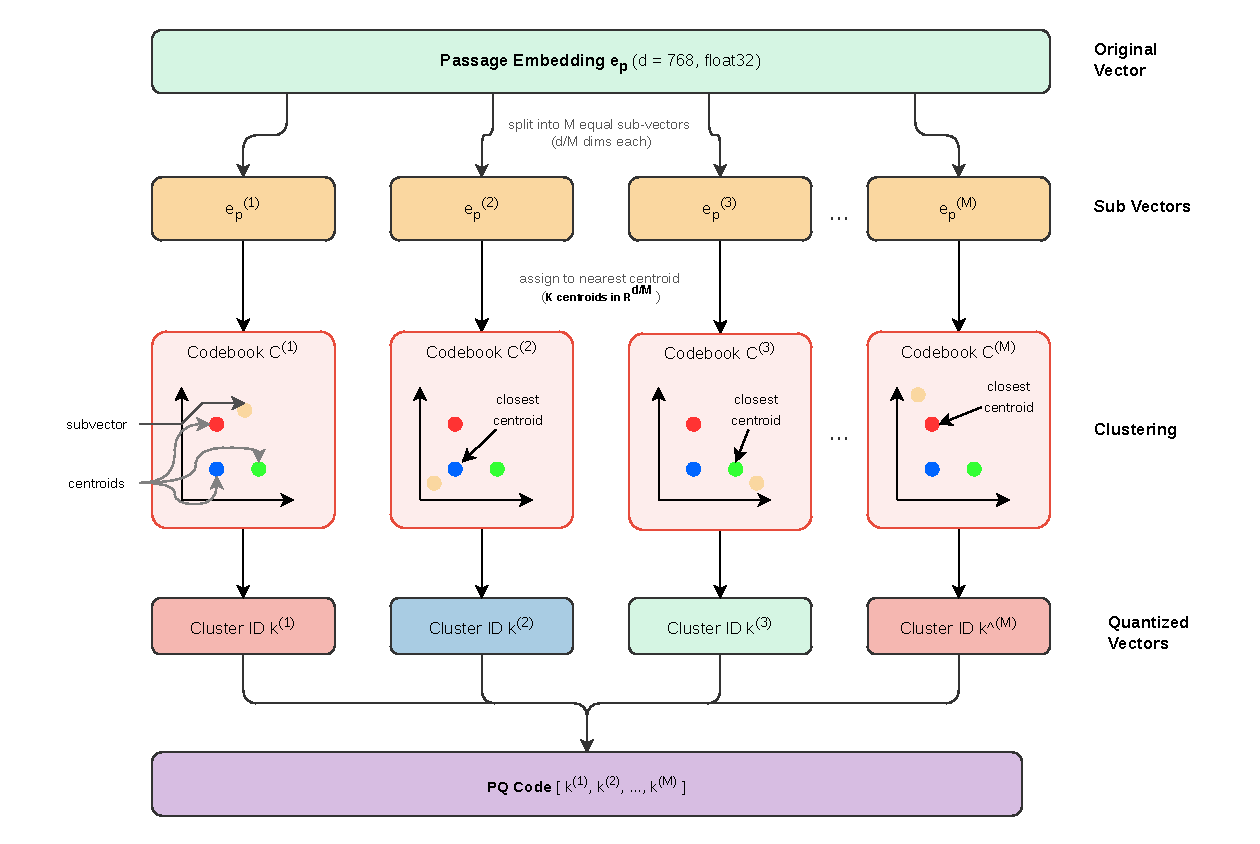
\includegraphics[width=0.85\textwidth]{Figures/pq.pdf}
  \caption[Product quantization (PQ) encoding pipeline.]{Product quantization encoding pipeline. Each passage embedding $\mathbf{e}_p \in \mathbb{R}^d$ is split into $M$ equally sized sub-vectors. The sub-vector is assigned to the closest centroid in its sub-space codebook. The codebook is fitted offline using $k$-means on the corpus. The compact PQ code is made up of the $M$ centroid indices. It cuts storage space from $d \times 4$ bytes to $M \times \lceil \log_2 K \rceil$ bits.}
  \label{fig:pq}
\end{figure}

High compression is possible with product quantization (PQ)~\cite{jegou2010product}. It does this by splitting each $d$-dimensional embedding into $M$ equal sub-vectors and giving each sub-vector a single integer number instead of raw floats. The full encoding process is shown in Figure~\ref{fig:pq}. A set of $K$ centroids is fit to the text embeddings by $k$-means for each of the $M$ subspaces. Then, the value of the closest centroid is put in place for each corpus sub-vector $\mathbf{e}^{(m)} \in \mathbb{R}^{d/M}$:
%
\begin{equation}
  \hat{k}^{(m)} = \operatorname*{arg\,min}_{k} \left\|\mathbf{e}^{(m)} - \mathbf{c}_k^{(m)}\right\|.
\end{equation}
%
A passage is saved as a list of $M$ numbers $(\hat{k}^{(1)}, \ldots, \hat{k}^{(M)})$, and each one needs $\log_2 K$ bits. A float32 embedding with 768 dimensions goes from 3,072 bytes to 64 bytes when $M = 64$ sub-vectors and $K = 256$ centroids. This is a compression ratio of $48\times$.

When the data are retrieved, the learned centroids are used to decode the corpus embeddings from their PQ codes back to their approximate float32 representations. Query embeddings, on the other hand, are kept at full float32 precision. After that, scoring is done by finding the standard cosine similarity between the rebuilt corpus and the query vectors. Asymmetric reconstruction, which only compresses the passage side and keeps the query accurate, brings back a lot of the quality that was lost during compression~\cite{johnson2021billion}.

\subsubsection{TurboQuant}

TurboQuant~\cite{zandieh2025turboquant} is a post-hoc method for reducing precision that works through three stages to get near-optimal rate-distortion performance. In the first stage, each embedding is rotated randomly (random Hadamard transform, $O(d \log d)$). The rotation keeps all pairwise distances and inner products the same, but the distribution of each coordinate transforms to a beta distribution, which means we can use a single quantizer for all dimensions. Second, a Lloyd-Max quantizer sets non-uniform bucket boundaries that reduce the mean squared error (MSE), bringing distortion within 2.7 times the Shannon lower bound. Third, because Lloyd-Max reconstruction introduces bias in inner product estimation, TurboQuant only allocates $b-1$ bits for MSE-optimal quantization and saves 1 bit for Quantized Johnson-Lindenstrauss (QJL). QJL fixes this bias. At retrieval time, the stored codes are decoded into nearby float32 vectors, and standard cosine similarity is used.

\begin{figure}[!h]
  \centering
  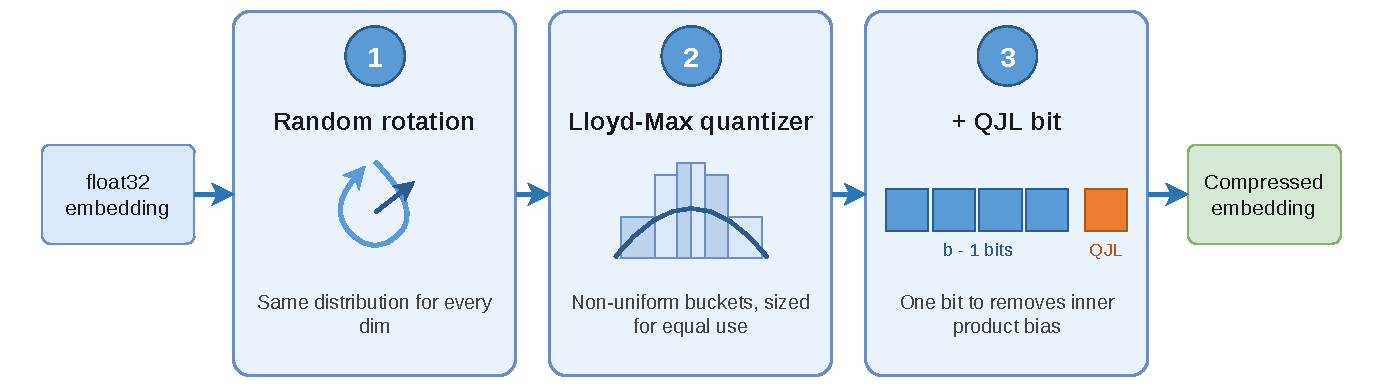
\includegraphics[width=0.95\textwidth]{Figures/tq.pdf}
  \caption[TurboQuant compression pipeline.]{The three stages of TurboQuant. A float32 embedding is first rotated randomly so every coordinate follows the same distribution, then quantized with a Lloyd-Max quantizer whose non-uniform buckets are sized for equal use, and finally one bit per code is reserved for the Quantized Johnson-Lindenstrauss (QJL) correction that removes the inner-product bias. The result is a compressed embedding.}
  \label{fig:turboquant}
\end{figure}

\subsection{Training-Time Methods}

\subsubsection{Straight-Through Estimator Binarization}

By adding the sign function to the model during fine-tuning, post-hoc binary quantization could be made a lot better. The main problem is that the sign function is not differentiable at zero and has zero derivative everywhere else. This means that normal backpropagation can't happen. To fix this, the Straight-Through Estimator (STE)~\cite{bengio2013estimating} uses the sign function in the forward pass and keeps the gradient the same in the backward pass, as if the operation were the identity function:
%
\begin{equation}
  \text{forward:} \quad \hat{\mathbf{e}} = \text{sign}(\mathbf{e}), \qquad \text{backward:} \quad \frac{\partial \mathcal{L}}{\partial \mathbf{e}} = \frac{\partial \mathcal{L}}{\partial \hat{\mathbf{e}}},
\end{equation}
%
where $\mathbf{e}$ is the embedding before binarization, and $\hat{\mathbf{e}}$ is its binarized form. There is a bias in the estimator because the passed gradient is not the true gradient of the sign function. However, \citeauthor{bengio2013estimating} report that it works better than more mathematically sound alternatives. When the STE is used to train the model, it encourages representations close to $\pm 1$. This way, the quantization step loses as little information as possible at the time of inference.

\subsubsection{Annealed Tanh Binarization}

The STE approximates the gradient of the sign function poorly. Annealed Tanh binarization replaces the STE with a smooth surrogate that gets sharper over time until it matches the sign function~\cite{cao2017hashnet}:
%
\begin{equation}
  \hat{\mathbf{e}} = \tanh(\beta \cdot \mathbf{e}),
\end{equation}
%
where $\beta$ is scheduled as $\beta_t = \sqrt{\gamma \cdot t + 1}$, $t$ is the global optimizer step and $\gamma$ is a growth rate hyperparameter~\cite{yamada2021efficient}. When training begins ($t = 0$), $\beta = 1$ and $\tanh(\mathbf{e}) \approx \mathbf{e}$ for small activations. This puts the model in a float32 domain with few restrictions. As training goes on, $\beta$ increases and $\tanh(\beta \cdot \mathbf{e})$ gets closer to $\text{sign}(\mathbf{e})$, making the binarization constraint tighter over time. The hard sign function is used at inference time to get back to a normal binary representation. The annealing schedule gives the model time to change how it represents things before the hard constraint is enforced. This progress is shown in Figure~\ref{fig:atanh} over six training stages.

\begin{figure}[!h]
  \centering
  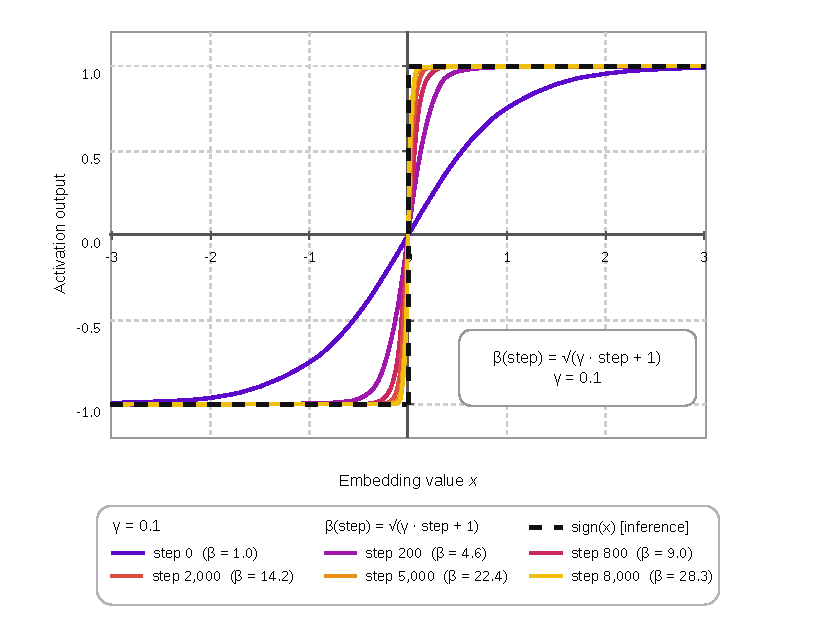
\includegraphics[width=0.85\textwidth]{Figures/atanh.pdf}
  \caption[Annealed Tanh binarization surrogate at six training checkpoints.]{Annealed Tanh binarization surrogate $\tanh(\beta_t \cdot x)$ at six training checkpoints with $\beta_t = \sqrt{\gamma \cdot t + 1}$ and $\gamma = 0.1$. At step 0 ($\beta = 1.0$), the surrogate is almost straight. At step 8{,}000 ($\beta = 28.3$, dashed), it becomes more like the hard sign function, which is used at inference time.}
  \label{fig:atanh}
\end{figure}

\subsubsection{Matryoshka Representation Learning}
\label{sec:mrl}

Matryoshka Representation Learning (MRL)~\cite{kusupati2022matryoshka} trains a model to concentrate the most important semantic information within the leading dimensions of the embedding vector. The main idea is that if you train the model to solve the retrieval task at different embedding truncation at the same time, the first few levels will pick up the most critical information, while the higher levels add more and more fine-grained details.

\begin{figure}[!h]
  \centering
  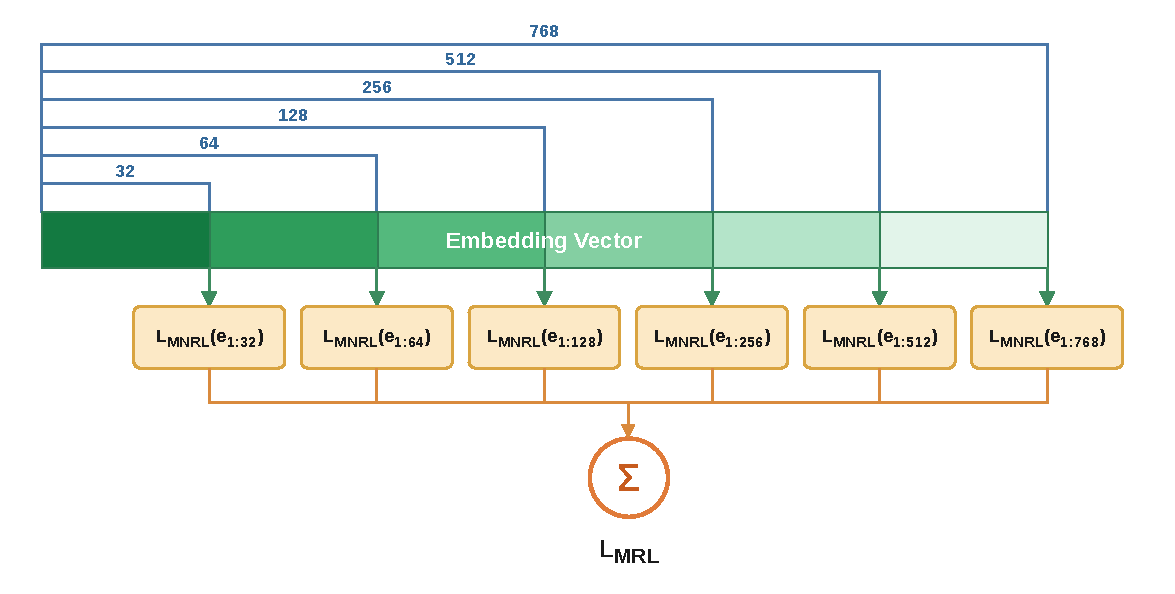
\includegraphics[width=0.9\textwidth]{Figures/mrl.pdf}
  \caption[Matryoshka Representation Learning (MRL) training.]{MRL training. Each prefix $\mathbf{e}_{1:m}$ for $m \in \mathcal{M} = \{32, 64, 128, 256, 512, 768\}$ is cut off from the passage embedding $\mathbf{e}_p \in \mathbb{R}^{768}$. There is a different MNRL loss for each truncation, and the total loss, $\mathcal{L}_{\text{MRL}}$, is equal to the sum of those losses (Equation~\ref{eq:mrl}).}
  \label{fig:mrl}
\end{figure}

As shown in Figure~\ref{fig:mrl}, MRL adds to the standard MNRL goal by computing losses at a fixed set of nested dimensions $\mathcal{M} = \{m_1, m_2, \ldots, m_K\}$, where $m_1 < m_2 < \cdots < m_K = d$. This is the multi-granularity loss:
%
\begin{equation}
  \mathcal{L}_{\text{MRL}} = \sum_{m \in \mathcal{M}} c_m \cdot \mathcal{L}_{\text{MNRL}}\!\left(\mathbf{e}_{1:m}\right),
  \label{eq:mrl}
\end{equation}
%
where $c_m$ are positive scalar weights. The MNRL loss $\mathcal{L}_{\text{MNRL}}(\mathbf{e}_{1:m})$ is found by using only the first $m$ dimensions. We use $\mathcal{M} = \{32, 64, 128, 256, 512, 768\}$ for all MRL studies in this thesis. The full embedding dimension is 768, which is equal to $d$.

At the time of inference, MRL lets the embedding be cut down to any number of dimensions ($m \in \mathcal{M} \setminus \{d\}$) without needing any extra fine-tuning. This makes it possible to directly reduce the number of dimensions at runtime. This is what makes MRL embeddings truly different from standard embeddings. Truncating a standard embedding will destroy the quality of the retrieval, but an MRL-trained embedding is made to stay useful at every supported truncation.

\section{Information Retrieval Evaluation}
\label{sec:ir_eval}

\subsection{Ranking Metrics}

Retrieval systems are evaluated by how well they rank relevant documents above irrelevant ones. All the metrics used in this thesis are based on the idea that each corpus document is either relevant to a given query or not. The retrieval system makes a ranked list of documents for each query. Metrics are calculated at cut-off $k$, which means that only the top $k$ documents in the ranked list are considered.

\textbf{Mean Reciprocal Rank (MRR@$k$)}~\cite{voorhees1999trec} is the primary metric used in this thesis. It measures the position of the first relevant document in the ranked list:
%
\begin{equation}
  \text{MRR}@k = \frac{1}{\text{rank}_1}, \quad
  \text{where } \text{rank}_1 = \min\{i \leq k : \text{doc}_i \in \mathcal{R}\},
  \label{eq:mrr}
\end{equation}
%
and $\text{MRR}@k = 0$ if the top $k$ doesn't have any relevant documents. MRR is very sensitive to the position of the single best hit, and it works well for retrieval tasks where there is only one right answer passage per query, which is the case for most NanoBEIR subsets.

\textbf{Normalized Discounted Cumulative Gain (NDCG@$k$)}~\cite{jarvelin2002cumulated} measures ranking quality by assigning higher credit to relevant documents appearing earlier in the list. The DCG at position $k$ is:
%
\begin{equation}
  \text{DCG}@k = \sum_{i=1}^{k} \frac{\mathbf{1}[\text{doc}_i \in \mathcal{R}]}{\log_2(i+1)},
  \label{eq:dcg}
\end{equation}
%
where $\mathcal{R}$ is the set of relevant documents and $\mathbf{1}[\cdot]$ is the indicator function. NDCG@$k$ normalizes DCG@$k$ by the ideal DCG (IDCG@$k$), which is the score that you get when all relevant documents are ranked first:
%
\begin{equation}
  \text{NDCG}@k = \frac{\text{DCG}@k}{\text{IDCG}@k}, \qquad
  \text{IDCG}@k = \sum_{i=1}^{\min(|\mathcal{R}|,\, k)} \frac{1}{\log_2(i+1)}.
  \label{eq:ndcg}
\end{equation}
%
NDCG@$k$ lies between 0 and 1, with 1 being the best possible score.

\textbf{Recall@$k$} is the fraction of the number of relevant documents that show up in the top $k$ results:
%
\begin{equation}
  \text{Recall}@k = \frac{|\{i \leq k : \text{doc}_i \in \mathcal{R}\}|}{|\mathcal{R}|}.
  \label{eq:recall}
\end{equation}
%
Recall@$k$ is limited by $\min(k, |\mathcal{R}|)/|\mathcal{R}|$ and only equals 1 when all relevant documents are found in the first $k$ positions.

All three metrics are computed at $k \in \{1, 3, 5, 10\}$, averaged over all queries in a NanoBEIR subset, and macro-averaged across the 13 subsets.

\subsection{Statistical Significance Testing}
\label{sec:significance_bg}

The retrieval benchmark has a fixed set of queries, and each can be scored by a model. Therefore, model comparison can be thought of as paired tests, which answer whether a model consistently outperforms another across the full set of queries.

\textbf{Shapiro--Wilk normality test}~\cite{shapiro1965analysis}. This test helps determine which significance test is reliable. It checks to see if the differences $\{d_i\}$ of scores follow a normal distribution.
\begin{itemize}
  \item $H_0$: the differences are normally distributed.
  \item $H_1$: the differences are not normally distributed.
\end{itemize}
If $H_0$ is rejected, the normality assumption of the paired $t$-test is broken, and the Wilcoxon test (non-parametric test) is the preferred choice.

\textbf{Paired $t$-test}~\cite{student1908probable}. A parametric test that assumes the differences are normally distributed and tests whether their mean is zero:
\begin{itemize}
  \item $H_0$: $\mu_d = 0$ (the two models have equal mean score).
  \item $H_1$: $\mu_d \neq 0$ (one model has a higher mean score).
\end{itemize}

\textbf{Wilcoxon signed-rank test}~\cite{wilcoxon1945individual}. A non-parametric test that does not assume normality and tests whether the median is zero. For each query, the difference $d_i$ is ranked by its magnitude. The test checks to see if the positive ranks (queries where model A wins) always beat the negative ranks (queries where model B wins):
\begin{itemize}
  \item $H_0$: the median difference is zero (neither model is better).
  \item $H_1$: the median difference is not zero.
\end{itemize}

\textbf{Cohen's $d$}~\cite{cohen1988statistical} quantifies the difference between two models:
%
\begin{equation}
  d = \frac{\bar{d}}{s_d}, \qquad
  \bar{d} = \frac{1}{n}\sum_{i=1}^{n} d_i, \qquad
  s_d = \sqrt{\frac{1}{n-1}\sum_{i=1}^{n}(d_i - \bar{d})^2}.
  \label{eq:cohens_d}
\end{equation}
%
Values of $|d| \approx 0.2$, $0.5$, and $0.8$ are conventionally interpreted as small, medium, and large effects, respectively.

\section{Related Work}
\label{sec:related}

The post-hoc methods described in Section~\ref{sec:compression_bg} are already practical at scale. The Hugging Face embedding quantization survey~\cite{shakir2024embedding} showed that post-hoc binary and INT8 quantization retain strong MTEB quality. This demonstrated that compressed embeddings can be used for large-scale retrieval without retraining. However, it was not clear if training-time methods can do better with the same or less memory.

Bengio \textit{et al.}~\cite{bengio2013estimating} came up with the idea for the STE (Section~\ref{sec:compression_bg}) for estimating gradients through stochastic neurons. Later, Courbariaux \textit{et al.}~\cite{courbariaux2016bnn} established it as a standard for binarizing neural network weights and activations. The annealed tanh alternative originated in HashNet~\cite{cao2017hashnet} for deep hashing. Beyond binary quantization, Yang \textit{et al.}~\cite{yang2019quantization} represent a $k$-level quantizer as a sum of $k{-}1$ shifted sigmoid functions with learnable biases. Shah \textit{et al.}~\cite{shah2024decoupled} reduce STE bias with separate forward and backward temperatures. Schr{\"o}dter \textit{et al.}~\cite{schrodter2025trainable} apply a similar sigmoid staircase to input feature compression. None of these multi-bit or decoupled variants have been applied to retrieval embeddings; they remain a natural direction for future work.

Both STE and annealed tanh have been adopted for dense retrieval. Yamada \textit{et al.}~\cite{yamada2021efficient} used annealed tanh in the Binary Passage Retriever (BPR). BPR achieves a $32\times$ memory reduction from 65~GB to 2~GB with zero accuracy loss on Natural Questions and TriviaQA. It uses binary Hamming search for candidate generation, followed by float32 reranking. It was trained with a joint margin ranking and MNRL loss. At production scale, Gan \textit{et al.}~\cite{gan2023binary} deployed recurrent residual binarization with STE at Tencent. Their approach stacks multiple binary stages to reach a user-specified bit depth at runtime. They report 30--50\% index cost savings in web search, video retrieval, and copyright detection. In our prior work, Pantha \textit{et al.}~\cite{pantha2026indussde} compared the post-hoc binarization with an embedding quantization-aware training method (BAT-STE). It demonstrated that quantization-aware training recovered most of the quality lost by naive post-hoc binarization at the same storage cost. But that comparison was limited to one model and one domain-specific benchmark. These results show that training-time compression can deliver better retrieval quality. However, each study has a different base model, training data, and benchmark, which makes the comparison difficult to judge. STE and annealed tanh have never been compared directly under identical conditions. In this thesis we make a direct comparison between them.

MRL (Section~\ref{sec:mrl}) is now prominent on the MTEB leaderboard~\cite{muennighoff2022mteb} and is a good choice when deployments have different memory budgets. SMEC~\cite{smec2025} identifies three problems with standard MRL: gradient fluctuation from optimizing shared encoder weights at the same time from different dimension losses; information loss from blind truncation; and weak contrastive learning from easy in-batch negatives. They solve it by sequential dimension training, adaptive dimension selection, and cross-batch memory. These changes improved the BEIR NDCG@10 score by 1.9 points at 128 dimensions. QAMA~\cite{qama2025} combines MRL with multi-level quantization-aware training. It uses learnable thresholds and a hybrid precision method. Hybrid precision involves using 2 bits for the first 25\% of dimensions and 0.5 bits for the last 25\%. This gives an effective 1.625~bits per dimension while keeping 95--98\% of the full-precision NDCG@10. The method only tests on ModernBERT and MiniLM, so it doesn't show how well it works on other architectures.

CoRECT~\cite{correct2025} provides the most comprehensive comparison of post-hoc methods to date. Its primary focus is on how retrieval performance degrades as corpus size scales from 10K to 100M passages. It evaluates eight techniques with four embedding models. It also presents the retrieval performance at various compression ratios for post-hoc methods. They found that quantization performs better than truncation at equal ratios, MRL training matters for truncation quality, and combining quantization with moderate truncation achieves the best scores for most models. CoRECT is the closest prior work in evaluation to this thesis, but it leaves training-time methods entirely out of scope.

No existing study enables a direct comparison between post-hoc and training-time compression under controlled conditions across multiple backbones. Most prior studies evaluate a limited set of backbone models, leaving open whether compression trade-offs generalize across architectures of different retrieval starting quality. Stacked combinations involving training-time methods remain unstudied. This thesis addresses all three gaps. In this thesis, all compression variants share the same pre-trained float32 baseline. Post-hoc methods use the fine-tuned float32 model, and training-time methods are fine-tuned with compression awareness on the same corpus and evaluated on NanoBEIR~\cite{nanobeir2024, thakur2021beir}. These experiments were repeated with three backbones: BGE-base-en-v1.5, RoBERTa-base, and MPNet-base to check the generalizability.

\begin{figure}[!h]
  \centering
  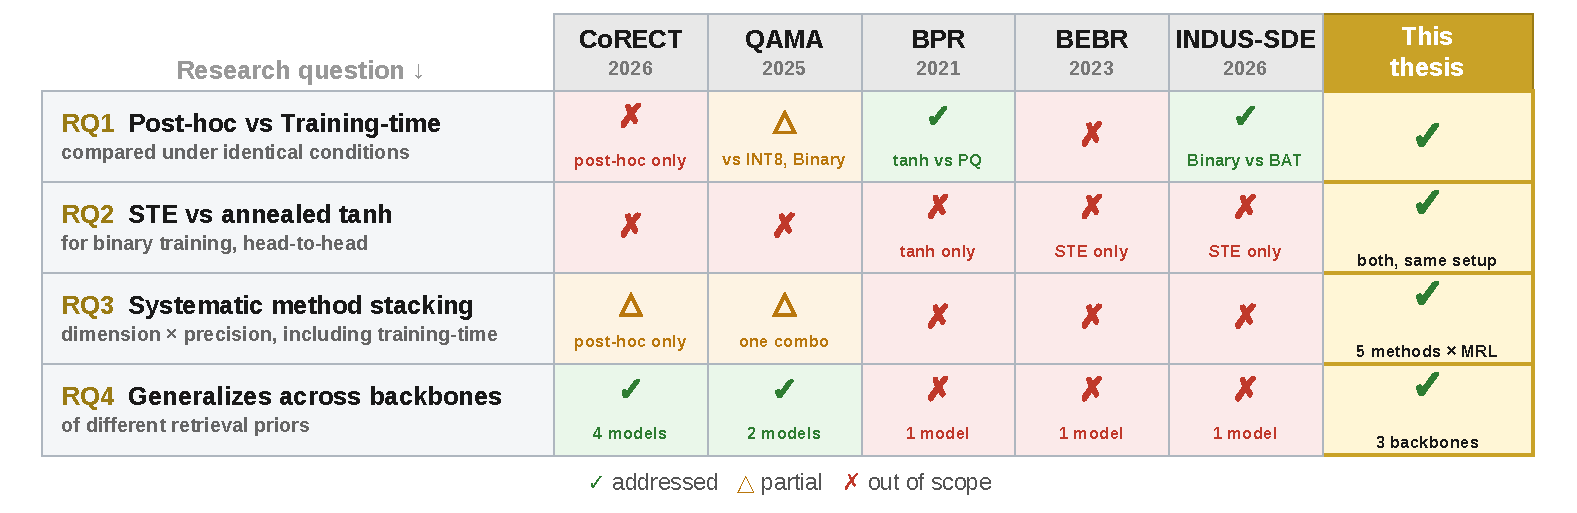
\includegraphics[width=\textwidth]{Figures/gap_matrix.pdf}
  \caption[Research gap matrix against representative prior work.]{Coverage of the four research questions across representative prior work, discussed above in this section. A check mark means the question is addressed, a triangle means it is partially addressed, and a cross means it is out of scope. No single prior study covers all four questions, which the experiments in this thesis address jointly.}
  \label{fig:gap_matrix}
\end{figure}
